\chapter{FET projects and social media}
Lorem ipsum dolor sit amet, consectetur adipisci elit, sed eiusmod tempor incidunt ut labore et dolore magna aliqua. Ut enim ad minim veniam, quis nostrum exercitationem ullam corporis suscipit laboriosam, nisi ut aliquid ex ea commodi consequatur. Quis aute iure reprehenderit in voluptate velit esse cillum dolore eu fugiat nulla pariatur. Excepteur sint obcaecat cupiditat non proident, sunt in culpa qui officia deserunt mollit anim id est laborum.

\section{Considered channels} 
An overview of the communication strategies adopted by FET projects on the web is provided by the fraction of projects which opened accounts on the most popular social media. For this thesis, the following communication channels were considered:

\begin{itemize}
 \item Website
 \item Twitter
 \item Facebook
 \item LinkedIn
 \item YouTube
 \item ResearchGate
\end{itemize}

Lorem ipsum dolor sit amet, consectetur adipisci elit, sed eiusmod tempor incidunt ut labore et dolore magna aliqua. Ut enim ad minim veniam, quis nostrum exercitationem ullam corporis suscipit laboriosam, nisi ut aliquid ex ea commodi consequatur. Quis aute iure reprehenderit in voluptate velit esse cillum dolore eu fugiat nulla pariatur. Excepteur sint obcaecat cupiditat non proident, sunt in culpa qui officia deserunt mollit anim id est laborum.

\begin{figure}[!t] 
 \begin{center}
 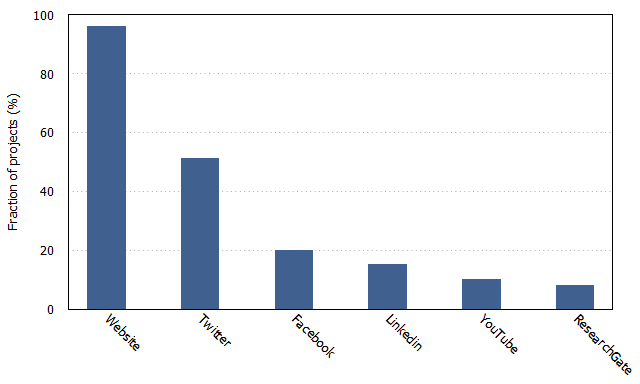
\includegraphics[scale=0.4]{Images/Social_media.png}
 \caption{Duration and allocated budget of Europe's Research and Innovation programmes (also known as Framework Programmes, FP). Budgets are expressed in billion Euros.}
 \label{FP_funds}
 \end{center}
\end{figure}